\documentclass[compress]{beamer}
\usepackage{irbookslide}
\usepackage{irilmenau2}
\usepackage{tikz}
\usepackage{url}
\usepackage{ifxetex}
%\RequireXeTeX
\usepackage{fontspec} % zahteva paket euenc
\usepackage{xunicode}
\usepackage{xltxtra}
\usepackage{polyglossia}
\usepackage{minted}
\usepackage[noend]{algorithmic}
\renewcommand{\algorithmicrequire}{\textbf{Input:}}
\renewcommand{\algorithmicensure}{\textbf{Output:}}
\usepackage{xcolor,colortbl}
\usepackage{textcomp}
\usepackage{unicode-math}
%\setdefaultlanguage[script=Latin]{serbian}

\title{Liste}
\author{\textcopyright \ \ Goodrich, Tamassia, Goldwasser}
\institute{Katedra za informatiku, Fakultet tehničkih nauka, Univerzitet u
Novom Sadu}
\date{2014.}
\subject{Predavanja sa ASP}

\begin{document}

\frame{\titlepage}

\section[1-Lista]{Jednostruko spregnuta lista}
\begin{frame}[fragile]
  \frametitle{Jednostruko spregnuta lista}
  \begin{itemize}
    \item predstavlja sekvencu elemenata
    \item elementi su sadržani u ,,čvorovima`` liste (nodes)
    \item susedstvo između elemenata se opisuje vezama/referencama/pokazivačima
    \item svaki čvor sadrži
    \begin{itemize}
      \item podatak koji se čuva
      \item link prema sledećem čvoru
    \end{itemize}
  \end{itemize}
  \begin{center}
    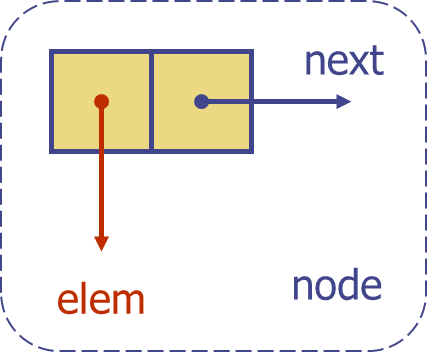
\includegraphics[width=3cm]{asp-07-pic01.png}
  \end{center}
\end{frame}

\begin{frame}[fragile]
  \frametitle{Jednostruko spregnuta lista}
  \begin{itemize}
    \item čvorovi ne zauzimaju susedne memorijske lokacije -- mogu biti ,,razbacani`` po memoriji
    \item redosled se održava pomoću veza između čvorova
    \item svaki čvor ima vezu prema sledećem
    \item koji je prvi?
    \begin{itemize}
      \item potrebna nam je posebna referenca na prvi element liste (,,glava``)
    \end{itemize}
    \item na koga pokazuje poslednji element?
    \begin{itemize}
      \item njegova referenca na sledećeg je None
    \end{itemize}
  \end{itemize}
  \begin{center}
    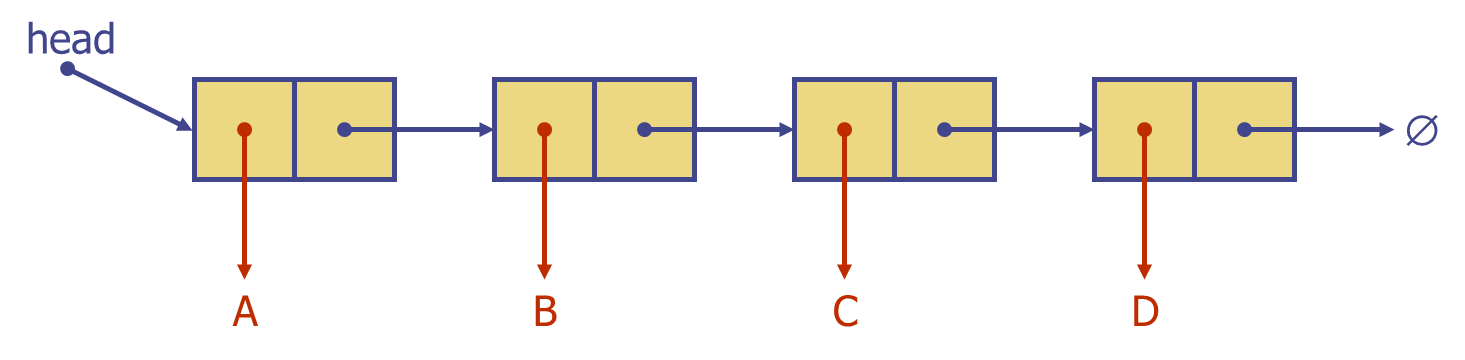
\includegraphics[width=11cm]{asp-07-pic02.png}
  \end{center}
\end{frame}

\begin{frame}[fragile]
  \frametitle{Element jednostruko spregnute liste u Pythonu}
\begin{minted}[linenos=false]{python}
class Node:
  def __init__(self, element, next):
    self._element = element
    self._next = next
\end{minted}
  \begin{center}
    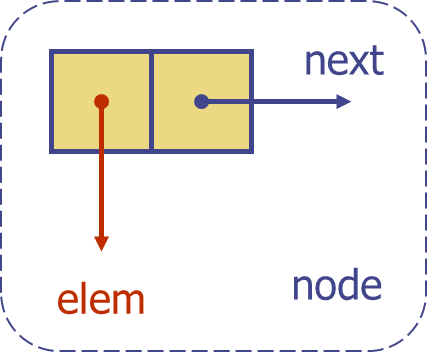
\includegraphics[width=3cm]{asp-07-pic01.png}
  \end{center}
\end{frame}

\section[Operacije]{Operacije nad jednostruko spregnutom listom}
\begin{frame}[fragile]
  \frametitle{Iterator: obilazak svih elemenata liste}
\begin{algorithmic}
\STATE $current \leftarrow head$
\WHILE{$current$ is not None}
  \STATE obradi $current$
  \STATE $current \leftarrow current.\_next$
\ENDWHILE
\end{algorithmic}
  \begin{center}
    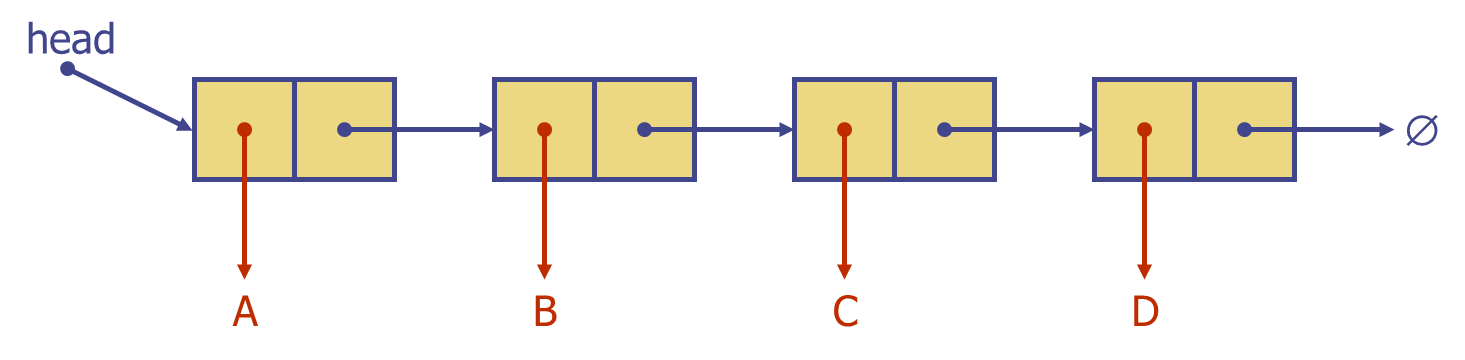
\includegraphics[width=11cm]{asp-07-pic02.png}
  \end{center}
\end{frame}

\begin{frame}[fragile]
  \frametitle{Poslednji element liste}
  \begin{itemize}
    \item kako doći do \textbf{poslednjeg} elementa liste?
    \begin{itemize}
      \item krenemo od glave dok ne dođemo do elementa čiji \texttt{\_next} je \texttt{None}
      \item ovaj postupak je $O(n)$
    \end{itemize}
    \item bilo bi zgodno čuvati referencu na poslednji element liste
    \begin{itemize}
      \item analogno glavi, referenca se zove ,,rep`` (tail)
    \end{itemize}
  \end{itemize}
  \begin{center}
    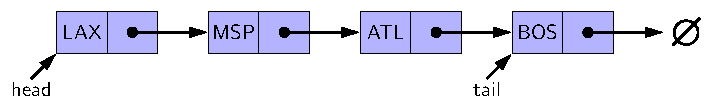
\includegraphics[width=10cm]{asp-07-pic02a.pdf}
  \end{center}
\end{frame}

\begin{frame}[fragile]
  \frametitle{Granični slučajevi}
  \begin{itemize}
    \item kako predstaviti praznu listu?
    \begin{itemize}
      \item \texttt{head = tail = None}
    \end{itemize}
    \item kako predstaviti punu listu?
    \begin{itemize}
      \item lista nema ograničenje na maksimalan broj elemenata :)
    \end{itemize}
    \item ako lista ima jedan element?
    \begin{itemize}
      \item \texttt{head == tail}
    \end{itemize}
  \end{itemize}
\end{frame}

\begin{frame}[fragile]
  \frametitle{Dodavanje elementa na početak liste}
  \begin{itemize}
    \item[1] kreiraj novi čvor
    \item[2] upiši podatak u čvor
    \item[3] link na sledeći novog čvora pokazuje na glavu
    \item[4] glava pokazuje na novi čvor
  \end{itemize}
  \begin{center}
    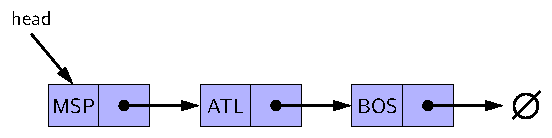
\includegraphics[scale=0.7]{asp-07-pic03a.pdf} \\
    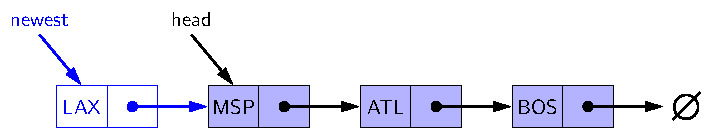
\includegraphics[scale=0.7]{asp-07-pic03b.pdf} \\
    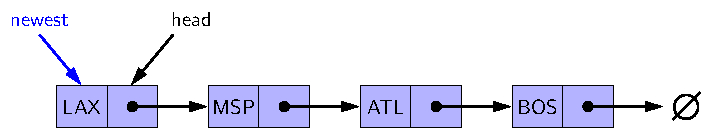
\includegraphics[scale=0.7]{asp-07-pic03c.pdf}
  \end{center}
\end{frame}

\begin{frame}[fragile]
  \frametitle{Dodavanje elementa na kraj liste}
  \begin{itemize}
    \item[1] kreiraj novi čvor
    \item[2] upiši podatak u čvor
    \item[3] link na sledeći novog čvora je \texttt{None}
    \item[4] poslednji$\rightarrow$sledeći pokazuje na novi čvor
    \item[5] \texttt{tail} pokazuje na novi čvor
  \end{itemize}
  \begin{center}
    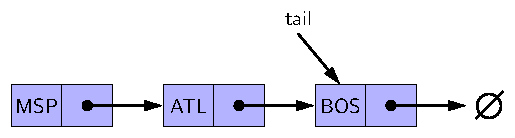
\includegraphics[scale=0.7]{asp-07-pic04a.pdf} \\
    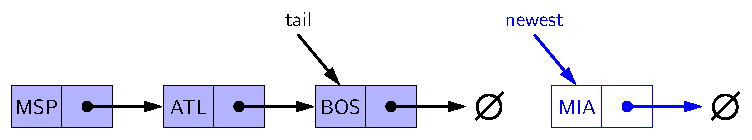
\includegraphics[scale=0.7]{asp-07-pic04b.pdf} \\
    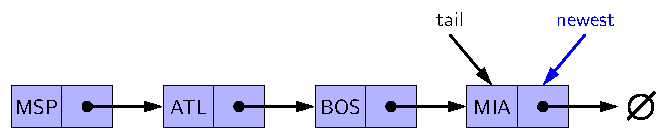
\includegraphics[scale=0.7]{asp-07-pic04c.pdf}
  \end{center}
\end{frame}

\begin{frame}[fragile]
  \frametitle{Uklanjanje elementa sa početka liste}
  \begin{itemize}
    \item[1] \texttt{head} treba da pokazuje na drugi element liste \\
    \texttt{head = head.\_next}
  \end{itemize}
  \begin{center}
    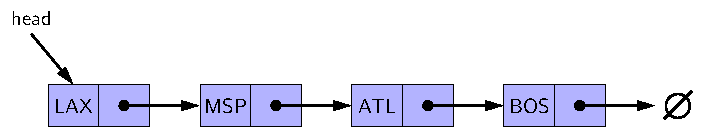
\includegraphics[scale=0.7]{asp-07-pic05a.pdf} \\
    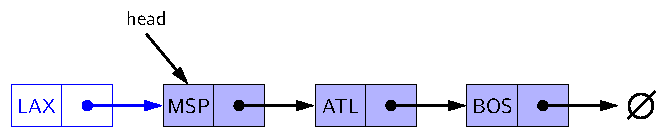
\includegraphics[scale=0.7]{asp-07-pic05b.pdf} \\
    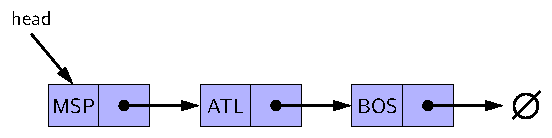
\includegraphics[scale=0.7]{asp-07-pic05c.pdf}
  \end{center}
\end{frame}

\begin{frame}[fragile]
  \frametitle{Uklanjanje elementa sa kraja liste}
  \begin{itemize}
    \item za vežbu ;)
  \end{itemize}
\end{frame}

\begin{frame}[fragile,shrink]
  \frametitle{Implementacija jednostruko spregnute liste u Pythonu $_1$}
\begin{minted}[linenos=false]{python}
class SingleList:
  def __init__(self):
    self._head = self._tail = None
  
  def add_first(self, elem):
    newest = Node(elem, self._head)
    self._head = newest
    if self._tail is None:     # ako je bila prazna 
      self._tail = self._head  # sada ima jedan element
    
  def add_last(self, elem):
    newest = Node(elem, None)
    if self._tail is not None:
      self._tail._next = newest
    self._tail = newest
    if self._head is None:     # ako je bila prazna
      self._head = newest      # sada ima jedan element
\end{minted}
\end{frame}

\begin{frame}[fragile,shrink]
  \frametitle{Implementacija jednostruko spregnute liste u Pythonu $_2$}
\begin{minted}[linenos=false]{python}
  def remove_first(self):
    if self._head is None:   # već je prazna
      return
    if self._head == self._tail:
      self._head = self._tail = None
    self._head = self._head._next
    
  def remove_last(self):
    if self._tail is None:
      return
    if self._head == self._tail:
      self._head = self._tail = None
    current = self._head
    while current._next != self._tail:
      current = current._next
    current._next = None
    self._tail = current
\end{minted}
\end{frame}

\begin{frame}[fragile,shrink]
  \frametitle{Implementacija jednostruko spregnute liste u Pythonu $_3$}
\begin{minted}[linenos=false]{python}
  def get_first(self):
    if self._head is not None:
      return self._head._element
    else:
      return None
        
  def get_last(self):
    if self._tail is not None:
      return self._tail._element
    else:
      return None
  
  def __len__(self):
    # ???
\end{minted}
\end{frame}

\section[2-Lista]{Dvostruko spregnuta lista}
\begin{frame}[fragile]
  \frametitle{Dvostruko spregnuta lista}
  \begin{itemize}
    \item kretanje ,,unazad`` (od repa prema glavi) u jednostruko spregnutoj listi je nemoguće
    \item rešenje: čvorovi treba da sadrže referencu i na prethodni i na sledeći element liste
  \end{itemize}
  \begin{center}
    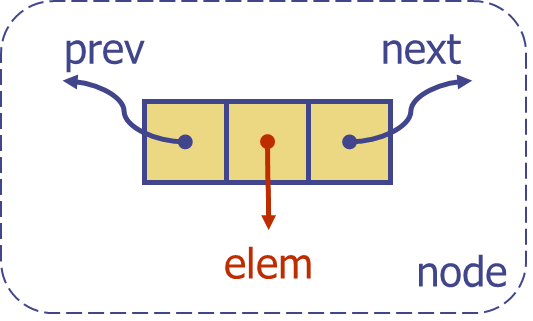
\includegraphics[width=5cm]{asp-07-pic06.png}
  \end{center}
\end{frame}

\begin{frame}[fragile]
  \frametitle{Element dvostruko spregnute liste u Pythonu}
\begin{minted}[linenos=false]{python}
class Node2:
  def __init__(self, element, prev, next):
    self._element = element
    self._prev = prev
    self._next = next
\end{minted}
\end{frame}

\begin{frame}[fragile]
  \frametitle{Dvostruko spregnuta lista: glava i rep}
  \begin{itemize}
    \item prvi i poslednji element imaju poseban status
    \item ne koriste se za čuvanje podataka
    \item prazna lista: \texttt{head.next == tail and tail.prev == head}
  \end{itemize}
  \begin{center}
    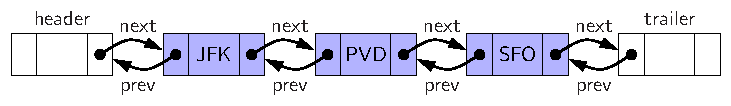
\includegraphics[width=10cm]{asp-07-pic07.pdf}
  \end{center}
\end{frame}

\section[Operacije]{Operacije nad dvostruko spregnutom listom}
\begin{frame}[fragile]
  \frametitle{Ubacivanje elementa u listu}
  \begin{center}
    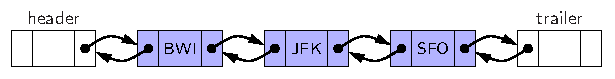
\includegraphics[scale=0.9]{asp-07-pic08a.pdf} \\
    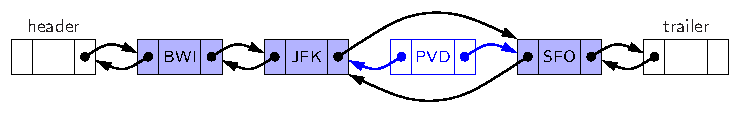
\includegraphics[scale=0.9]{asp-07-pic08b.pdf} \\
    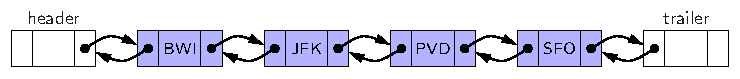
\includegraphics[scale=0.9]{asp-07-pic08c.pdf}
  \end{center}
\end{frame}

\begin{frame}[fragile]
  \frametitle{Dodavanje elementa na početak liste}
  \begin{center}
    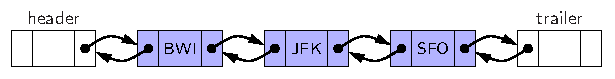
\includegraphics[scale=0.9]{asp-07-pic09a.pdf} \\
    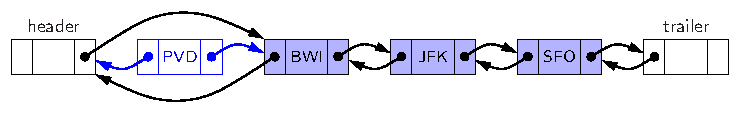
\includegraphics[scale=0.9]{asp-07-pic09b.pdf} \\
    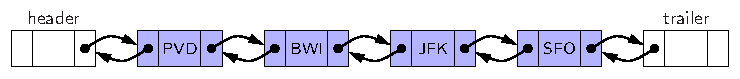
\includegraphics[scale=0.9]{asp-07-pic09c.pdf}
  \end{center}
\end{frame}

\begin{frame}[fragile]
  \frametitle{Uklanjanje elementa iz liste}
  \begin{center}
    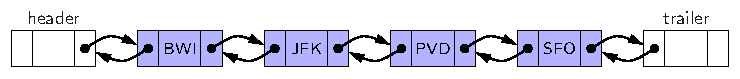
\includegraphics[scale=0.9]{asp-07-pic10a.pdf} \\
    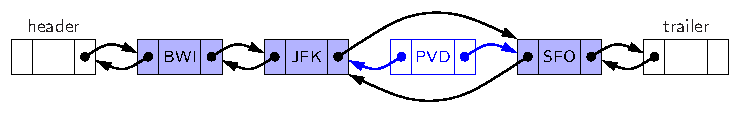
\includegraphics[scale=0.9]{asp-07-pic10b.pdf} \\
    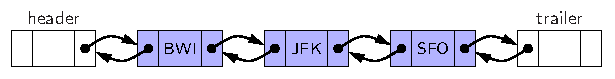
\includegraphics[scale=0.9]{asp-07-pic10c.pdf}
  \end{center}
\end{frame}

\begin{frame}[fragile,shrink]
  \frametitle{Dvostruko spregnuta lista u Pythonu}
\begin{minted}[linenos=false]{python}
class DoubleList:
  def __init__(self):
    self._head = self.Node2(None, None, None)
    self._tail = self.Node2(None, None, None)
    self._head._next = self._tail
    self._tail._prev = self._head

  def is_empty(self):
    return self._head._next == self._tail
    
  def insert_before(self, element, successor):
    newest = self.Node2(element, successor._prev, successor)
    successor._prev._next = newest
    successor._prev = newest
    return newest
    
  def delete(self, node):
    if self.is_empty():
      return
    predecessor = node._prev
    successor = node._next
    predecessor._next = succesor
    element = node._element
    node._prev = node._next = node._element = None
    return element
\end{minted}
\end{frame}

\end{document}
